\section*{Đề thi thử Sở giáo dục sơn la 25-26 Lần 3}
\begin{ex} %Câu 1
	Họ tất cả các nguyên hàm của hàm số $f(x)=\mathrm{e}^x+\sin x$ là
	\choice
	{$\mathrm{e}^x+\sin x+C$}
	{\True $\mathrm{e}^x-\cos x+C$}
	{$\mathrm{e}^x-\sin x+C$}
	{$\mathrm{e}^x+\cos x+C$}
	\loigiai{
	}
\end{ex}
\begin{ex} %Câu 2
	Thời gian hoàn thành một câu hỏi trả lời ngắn (đơn vị là phút) của học sinh nữ lớp 12 A thu được kết quả thống kê như sau:
	\begin{center}
		\begin{tabular}{|c|c|c|c|c|c|}
			\hline
			Thời gian (phút) & $[0;4)$ & $[4;8)$ & $[8;12)$ & $[12;16)$ & $[16;20)$ \\
			\hline
			Số học sinh & $2$ & $4$ & $7$ & $4$ & $3$ \\
			\hline
		\end{tabular}
	\end{center}
	Khoảng biến thiên của mẫu số liệu trên bằng
	\choice
	{$10$}
	{$16$}
	{\True $20$}
	{$4$}
	\loigiai{
	}
\end{ex}
\begin{ex} %Câu 3
	Cho cấp số nhân $\left(u_n\right)$ có số hạng đầu $u_1=2$ và công bội $q=5$. Giá trị của $u_3$ bằng
	\choice
	{$10$}
	{$12$}
	{$7$}
	{\True $50$}
	\loigiai{
	}
\end{ex}
\begin{ex} %Câu 4
	Nghiệm của phương trình $4^{x+2}=64$ là
	\choice
	{$0$}
	{$3$}
	{$2$}
	{\True $1$}
	\loigiai{
	}
\end{ex}
\begin{ex} %Câu 5
	\immini{
	Cho hình hộp $ABCD.A'B'C'D'$ (tham khảo hình vẽ).
	Khẳng định nào sau đây đúng?
	\choice
	{$\overrightarrow{AB}+\overrightarrow{AD}+\overrightarrow{A'A}=\overrightarrow{AC'}$}
	{\True $\overrightarrow{AB}+\overrightarrow{AD}+\overrightarrow{AA'}=\overrightarrow{AC'}$}
	{$\overrightarrow{AB}+\overrightarrow{AB'}+\overrightarrow{AA'}=\overrightarrow{AC'}$}
	{$\overrightarrow{AB}+\overrightarrow{AC}+\overrightarrow{AA'}=\overrightarrow{AC'}$}
}{
\begin{tikzpicture}[scale=0.7, font=\footnotesize,line join=round, line cap=round, >=stealth]
		\def\h{3}
		\path (0,0) coordinate (A)
		(-1.5,-1.2) coordinate (B)
		++(4,0) coordinate (C)
		($(A)+(C)-(B)$) coordinate(D);
		\foreach \i in {A,B,C,D} \path (\i)+(-0.5,\h) coordinate(\i');
		\draw (B')--(C')--(D')--(A')--(B') --(B)--(C)--(D)--(D') (C)--(C');
		\draw[dashed] (D)--(A)--(B) (A)--(A');
		\foreach \diem/\pos in {A/160, B/-135, C/-45, D/0, A'/135, B'/135, C'/90, D'/45} \fill (\diem) node[shift={(\pos:3mm)}] {$\diem$} circle(1pt);
\end{tikzpicture}
}
	\loigiai{
	}
\end{ex}
\begin{ex} %Câu 6
	Trong không gian $Oxyz$, cho mặt cầu $(S)\colon (x-3)^2+(y+2)^2+(z-1)^2=9$. Bán kính của $(S)$ bằng
	\choice
	{$9$}
	{$81$}
	{\True $3$}
	{$18$}
	\loigiai{
	}
\end{ex}
\begin{ex} %Câu 7
	Cho hình phẳng ($H$) giới hạn bởi các đường thẳng $y=x^3+x+2$, $y=0$, $x=0$, $x=2$. Gọi $V$ là thể tích của khối tròn xoay được tạo thành khi quay $(H)$ xung quanh trục $Ox$. Mệnh đề nào dưới đây đúng?
	\choice
	{\True $V=\pi \displaystyle\int\limits_0^2\left(x^3+x+2\right)^2\mathrm{d}x$}
	{$V=\pi \displaystyle\int\limits_0^2\left(x^3+x+2\right)\mathrm{d}x$}
	{$V=\displaystyle\int\limits_0^2\left(x^3+x+2\right)^2\mathrm{d}x$}
	{$V=\displaystyle\int\limits_0^2\left(x^3+x+2\right)\mathrm{d}x$}
	\loigiai{
	}
\end{ex}
\begin{ex} %Câu 8
	Phương trình $\sin x=1$ có tập nghiệm là
	\choice
	{$S=\{k\pi \mid k\in \mathbb{Z}\}$}
	{\True $S=\left\{\left.\dfrac{\pi}{2}+k2\pi \right\rvert\,k\in \mathbb{Z}\right\}$}
	{$S=\left\{\left.\dfrac{\pi}{2}+k\pi \right\rvert\,k\in \mathbb{Z}\right\}$}
	{$S=\{k2\pi \mid k\in \mathbb{Z}\}$}
	\loigiai{
	}
\end{ex}
\begin{ex} %Câu 9
	Tiệm cận đứng của đồ thị hàm số $y=\dfrac{x^2+4x+1}{x-1}$ là
	\choice
	{$x=-4$}
	{$x=4$}
	{\True $x=1$}
	{$y=1$}
	\loigiai{
	}
\end{ex}
\begin{ex} %Câu 10
	\immini{
	Cho hình chóp $S.ABCD$ có đáy là hình vuông, cạnh bên $SA$ vuông góc với đáy. Góc giữa đường thẳng $SC$ và mặt phẳng ($ABCD$) là góc nào sau đây?
	\choice
	{$\widehat{ASC}$}
	{$\widehat{SCB}$}
	{\True $\widehat{SCA}$}
	{$\widehat{SAC}$}
}{
\begin{tikzpicture}[line join=round,line cap=round,>=stealth,scale=.7,font=\footnotesize]
	\foreach \x/\y/\n in {0/0/A,-2/-1.5/D,4/0/B} \coordinate (\n) at (\x,\y);
	\coordinate (C) at ($(B)+(D)-(A)$);
	\coordinate (O) at ($(B)!0.5!(D)$);
	\coordinate (S) at ($(A)+(0,3)$);
	\coordinate (I) at ($(S)!0.5!(C)$);
	\draw (S)--(B)--(C)--(D)--(S)--(C);
	\draw[dashed] (S)--(A) (D)--(A)--(B);
	\foreach \t/\g in {S/90,A/170,D/-120,C/-30,B/30}{
		\fill (\t) circle (1pt) node[shift={(\g:8pt)}]{$ \t $};
	}
	\draw pic[thin,draw,angle radius=2mm] {right angle= S--A--B};
\end{tikzpicture}
}
	\loigiai{
	}
\end{ex}
\begin{ex} %Câu 11
	\immini{
	Hàm số nào dưới đây có đồ thị như hình vẽ?
	\choice
	{$y=\dfrac{x^2+3x-4}{x-2}$}
	{$y=x^3-3x^2-4$}
	{\True $y=-x^3+3x^2-4$}
	{$y=\dfrac{x-4}{x-1}$}
}{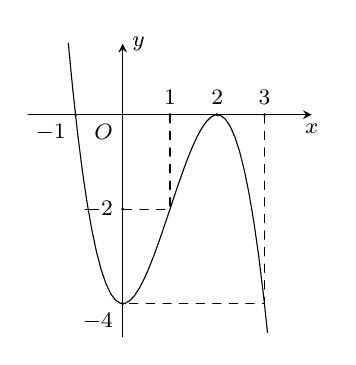
\begin{tikzpicture}[scale=0.6,>=stealth, font=\footnotesize, line join=round, line cap=round]
\draw[->] (-2,0)--(0,0) node[below left]{$O$}--(4,0) node[below]{$x$};
\draw[->] (0,-4.7)--(0,1.5) node[right]{$y$};
\clip (-2,1.5) rectangle (3.1,-4.6);
\draw[samples=100] plot(\x,{-1*(\x)^3+3*(\x)^2-4});
\fill[black] (0,-4)node[below left]{$-4$}circle(1pt)
(2,0)node[above]{$2$}circle(1pt)
(-1,0)node[below left]{$-1$}circle(1pt)
(1,0)node[above]{$1$}circle(1pt)
(3,0)node[above]{$3$}circle(1pt)
(0,-2)node[left]{$-2$}circle(1pt)
;
\draw[dashed] (3,0)|-(0,-4) (1,0)|-(0,-2);
\end{tikzpicture}
}
	\loigiai{
	}
\end{ex}
\begin{ex} %Câu 12
	Trong không gian $Oxyz$, vectơ chỉ phương của đường thẳng $(d)\colon\dfrac{x-2}{2}=\dfrac{y+1}{-1}=\dfrac{z-3}{1}$ là
	\choice
	{$\overrightarrow{u_3}=(2;-1;3)$}
	{$\overrightarrow{u_2}=(2;1;1)$}
	{\True $\overrightarrow{u_1}=(2;-1;1)$}
	{$\overrightarrow{u_4}=(-1;1;3)$}
	\loigiai{
	}
\end{ex}
\cauds
\begin{ex} %Câu 1
	Cho hàm số $y=\dfrac{2x^2-2x+2}{-x+1}$.
	\choiceTF
	{Hàm số nghịch biến trên khoảng $(-\infty,0)\cup(2;+\infty)$}
	{\True Hàm số đạt cực tiểu tại $x=0$}
	{Giá trị nhỏ nhất của hàm số trên đoạn $\left[\dfrac{3}{2};\dfrac{7}{2}\right]$ bằng $-7$}
	{\True Gọi $A$, $B$ là hai điểm cực trị của đồ thị hàm số. Cho điểm $M(-1;0)$, gọi $D(a;b)$ là chân đường phân giác trong góc $M$ của tam giác $MAB$. Khi đó $a+b=\dfrac{1}{2}$}
	\loigiai{
	}
\end{ex}
\begin{ex} %Câu 2
	Một vật trang trí có dạng một khối tròn xoay được tạo thành khi quay miền $(R)$ (phần tô đậm trong hình vẽ) quanh trục $MN$. Biết rằng $ABCD$ là hình chữ nhật với $AB=6$\,cm, $AD=10$\,cm và $M$, $N$ lần lượt là trung điểm của $AB,CD$. Hai đường cong là đường Elip có hình chữ nhật cơ sở là $ABCD$ và đường tròn tiếp xúc với hai cạnh $AD$ và $BC$. Gắn hệ tọa độ $Oxy$ (đơn vị trên mỗi trục là $1$\,cm) như hình vẽ.
\begin{center}
	\begin{tikzpicture}[scale=0.65,declare function={a=5; b=3;}]
		\path
		(0,0) coordinate (O)
		(-a,b) coordinate (A)
		(-a,-b) coordinate (B)
		(a,-b) coordinate (C)
		(a,b) coordinate (D)
		(-a,0) coordinate (M)
		(a,0) coordinate (N)
		(0,b) coordinate (P)
		(0,-b) coordinate (Q)
		(-b,0) coordinate (M1)
		(b,0) coordinate (N1)
		;
		\fill[pattern=north east lines](0,0) ellipse (a and b);
		\fill[white](0,0) circle (3);
		\draw[->] (-6,0)--(6,0)
		node[shift={(-100:7pt)},font=\normalsize]{$x$};
		\draw[->] (0,-4)--(0,4)
		node[shift={(180:7pt)},font=\normalsize]{$y$};
		\draw (0,0) ellipse (a and b);
		\draw (0,0) circle (3);
		\draw (-5,-3) rectangle (5,3);
		\foreach \p/\g in{A/135,B/-135,C/-45,D/45,M/140,N/40,O/-135}
		\draw[fill=white](\p) circle (.02)node[shift={(\g:.2)},scale=.7]{$\p$};
		\foreach \p/\g/\k in{P/135/3,Q/-135/-3,M/-135/-5,N/-45/5,M1/45/-3,N1/135/3}
		\draw[fill=white](\p) circle (.02)node[shift={(\g:.3)},scale=.7]{$\k$};
	\end{tikzpicture}
\end{center}
	\choiceTF
	{\True Đường tròn tâm $O$ tiếp xúc với hai cạnh $AD,BC$ có phương trình là $x^2+y^2=9$}
	{Phương trình của đường Elip có hình chữ nhật cơ sở là $ABCD$ là $\dfrac{x^2}{5}+\dfrac{y^2}{3}=1$}
	{Diện tích phần tô đậm là $S=\displaystyle\int\limits_{-5}^5\sqrt{9\left(1-\dfrac{x^2}{25}\right)}\mathrm{d}x-\displaystyle\int\limits_{-3}^3\sqrt{9-x^2}\mathrm{\,d}x$}
	{\True Thể tích của vật trang trí đó là $75,4$\,cm$^3$ (kết quả làm tròn đến)}
	\loigiai{
	}
\end{ex}
\begin{ex} %Câu 3
	Trong không gian với hệ trục tọa độ $Oxyz$, cho hai mặt cầu $(S)\colon (x-3)^2+y^2+z^2=9$; $(S')\colon x^2+y^2+z^2-12y+12=0$ và mặt phẳng $(P)\colon z-m=0$.
	\choiceTF
	{\True Mặt cầu $(S)$ có tâm là $I(3;0;0)$ và mặt cầu $(S')$ có bán kính là $\sqrt{24}$}
	{Mặt phẳng $(P)$ có một vectơ pháp tuyến là $\overrightarrow{n}=(1;0;0)$}
	{\True Khoảng cách giữa hai tâm của hai mặt cầu ($S$) và ($S'$) bằng $3\sqrt{5}$}
	{Biết rằng hai mặt cầu $(S)$ và $(S')$ cắt nhau theo giao tuyến là đường tròn $(C)$. Gọi $T$ là tập hợp các giá trị của $m$ để trên mặt phẳng $(P)$ dựng được một tiếp tuyến đến đường tròn $(C)$. Tổng bình phương các phần tử của tập hợp $T$ là $2$}
	\loigiai{
	}
\end{ex}
\begin{ex} %Câu 4
	Hai bạn An và Bình tham gia một buổi phỏng vấn tuyển cộng tác viên cho câu lạc bộ truyền thông của nhà trường. Ban xét tuyển có một hộp đựng $10$ câu hỏi thuộc lĩnh vực tự nhiên và $20$ câu hỏi thuộc lĩnh vực xã hội. An rút ngẫu nhiên $1$ câu hỏi (không bỏ lại vào hộp), sau đó Bình rút ngẫu nhiên $1$ câu hỏi.
	\choiceTF
	{\True Xác suất An rút được câu hỏi thuộc lĩnh vực tự nhiên là $\dfrac{1}{3}$}
	{Biết rằng An rút được câu hỏi thuộc lĩnh vực tự nhiên, xác suất Bình rút được câu hỏi thuộc lĩnh vực xã hội là $\dfrac{2}{3}$}
	{\True Xác suất Bình rút được câu hỏi thuộc lĩnh vực xã hội là $\dfrac{2}{3}$}
	{Biết rằng Bình rút được câu hỏi thuộc lĩnh vực xã hội, xác suất để An rút được câu hỏi thuộc lĩnh vực tự nhiên là $\dfrac{19}{29}$}
	\loigiai{
	}
\end{ex}
\caukq
\begin{ex} %Câu 1
	Cho hình chóp $S.ABCD$ có đáy $ABCD$ là hình thang vuông tại $A$ và $B$, $AB=BC=a$, $AD=2a$$, $ $SA$ vuông góc với đáy và $SA=a$. Gọi $M$, $N$ lần lượt là trung điểm của $SB$ và $CD$. Tính góc giữa $MN$ và $(SAC)$ theo đơn vị độ (kết quả làm tròn đến hàng đơn vị).
		\par
	\shortans{42}
	\loigiai{
	}
\end{ex}
\begin{ex} %Câu 2
	\immini{
	Khi chế tạo cánh diều hình tứ giác, người ta sẽ tạo khung trước. Một khung cánh diều sẽ được tạo từ hai thanh chéo làm bằng gỗ và bốn sợi dây cước viền. Lấy bốn sợi dây tạo thành viền ngoài đã được cắt đúng độ dài với kích thước là $40$, $40$$, $ $96$, $96$ (theo đơn vị cm) như hình vẽ và lắp hai thanh gỗ làm đường chéo. Tính tổng độ dài hai thanh chéo gỗ khi diện tích cánh diều lớn nhất (đơn vị cm, kết quả làm tròn đến hàng đơn vị).
}{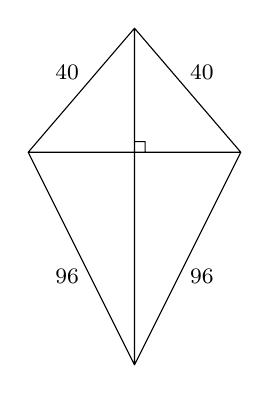
\begin{tikzpicture}[scale=.45, font=\footnotesize, line join=round, line cap=round, >=stealth]
	\draw (3,0)--(0,3.5)--(-3,0)--(0,-6)--cycle
	(0,3.5)--(0,-6) (3,0)--(-3,0)
	(0,.3)--(.3,.3)--(.3,0)
	;
	\node at(1.9,2.25){$40$};
	\node at(-1.9,2.25){$40$};
	\node at(1.9,-3.5){$96$};
	\node at(-1.9,-3.5){$96$};
	\end{tikzpicture}}
\par
\shortans{178}
	\loigiai{
	}
\end{ex}
\begin{ex} %Câu 3
	Cho tập hợp $S=\{1;2;3;\ldots;15\}$. Có bao nhiêu cách chọn ra $6$ số phân biệt từ tập $S$ và sắp xếp chúng thành một dãy $\left(a_1;a_2;a_3;a_4;a_5;a_6\right)$ thỏa mãn đồng thời hai điều kiện sau:
	\begin{itemize}
		\item Biểu thức $\log _3\left(a_1\right)+\log _3\left(a_2\right)+\log _3\left(a_3\right)$ là một số nguyên.
		\item $a_1+a_6=a_2+a_5=a_3+a_4$.
	\end{itemize}
		\par
	\shortans{30}
	\loigiai{
	}
\end{ex}
\begin{ex} %Câu 4
	Một khu vui chơi có sơ đồ như hình vẽ. Khách hàng xuất phát từ khu Trung tâm, đi qua các cánh cửa để tham quan các khu vực khác. Giá vé cho mỗi lần bước qua một cánh cửa (theo bất kỳ chiều nào) được ghi trên sơ đồ (đơn vị tiền là đồng). Sau khi đã đi qua tất cả các khu vực, khách hàng phải trở lại khu Trung tâm để ra ngoài. Hỏi khách hàng phải tốn ít nhất bao nhiêu nghìn đồng tiền mua vé?
	\begin{center}
		\begin{tikzpicture}[scale=1,>=stealth, line join=round, line cap=round]
		\draw 
		(-3,0)--(3,0)--(3,-5)--(-3,-5)--cycle 	(-3,-4)--(3,-4) (-1,0)--(-1,-4) (1,0)--(1,-4) (-1,-2.5)--(1,-2.5);
		\node[fill=white,inner sep=1pt,font=\footnotesize] at (0,0) {Cửa ra vào};
		\node[fill=white,inner sep=1pt,font=\footnotesize] at (0,-.75) {Trung tâm};
		\node[fill=white,inner sep=1pt,font=\footnotesize] at (0,-4) {$190\,000$};
		\node[fill=white,inner sep=1pt,font=\footnotesize] at (0,-2.5) {$80\,000$};
		\node[fill=white,inner sep=1pt,font=\footnotesize] at (-1,-1.25) {$170\,000$};
		\node[fill=white,inner sep=1pt,font=\footnotesize] at (1,-1.25) {$200\,000$};
		\node[fill=white,inner sep=1pt,font=\footnotesize] at (-1,-3.25) {$290\,000$};
		\node[fill=white,inner sep=1pt,font=\footnotesize] at (1,-3.25) {$90\,000$};
		\node[fill=white,inner sep=1pt,font=\footnotesize] at (-2,-4) {$120\,000$};
		\node[fill=white,inner sep=1pt,font=\footnotesize] at (2,-4) {$100\,000$};
		\end{tikzpicture}
	\end{center}
	\par
\shortans{560}
	\loigiai{
	}
\end{ex}
\begin{ex}%[12-EX-2-2025, Lương Như Quỳnh]%[2D4V3-2]
	Một khuôn viên dạng nửa hình tròn, trên đó người thiết kế phần để trồng hoa có dạng của một cánh hoa hình parabol có đỉnh trùng với tâm và có trục đối xứng vuông góc với đường kính của nửa hình tròn, hai đầu mút của cánh hoa nằm trên nửa đường tròn (phần tô màu) và cách nhau một khoảng bằng $4$ m. Phần còn lại của khuôn viên (phần không tô màu) dành để trồng cỏ Nhật Bản. Biết các kích thước cho như hình vẽ, chi phí để trồng hoa và cỏ Nhật Bản tương ứng là $150\,000$ đồng /m$^2$ và $100\,000$ đồng /m$^2$. Hỏi cần bao nhiêu tiền (triệu đồng) để trồng hoa và trồng cỏ Nhật Bản trong khuôn viên đó? \textit{(Số tiền được làm tròn đến hàng phần trăm)}
	\begin{center}
		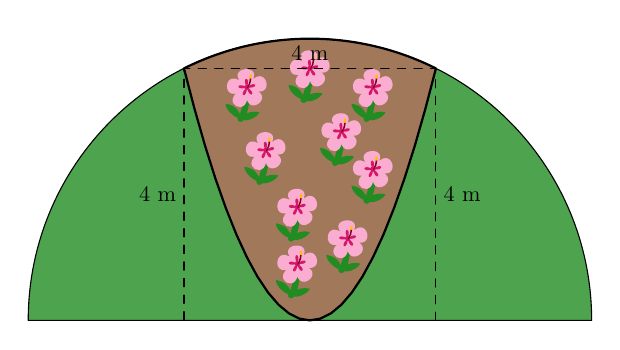
\begin{tikzpicture}[line join=round, line cap=round,scale=.8,transform shape]
			\definecolor{lavenderpink}{rgb}{0.98, 0.68, 0.82}
			\definecolor{dogwoodrose}{rgb}{0.84, 0.09, 0.41}
			\definecolor{burgundy}{rgb}{0.5, 0.0, 0.13}
			\definecolor{citrine}{rgb}{0.89, 0.82, 0.04}
			\definecolor{amber}{rgb}{1.0, 0.75, 0.0}
			\definecolor{forestgreen(web)}{rgb}{0.13, 0.55, 0.13}%màu lá
			\definecolor{chamoisee}{rgb}{0.63, 0.47, 0.35}
			%\clip (-4,-1) rectangle (4,4);
			
			\def\R{4}
			\pgfmathsetmacro{\r}{sqrt{20}}
			\path
			(0,0) coordinate (O);
			\def\xa{2}
			\def\ya{4}
			\def\xb{-2}
			\def\yb{4}
			\pgfmathsetmacro{\thetaA}{atan2(\ya,\xa)}
			\pgfmathsetmacro{\thetaB}{atan2(\yb,\xb)}
			
			\draw[fill=forestgreen(web)!80](\r,0) arc (0:180:\r)--cycle;
			\draw[thick, fill=chamoisee] (\thetaA:\r) arc (\thetaA:\thetaB:\r)--plot[domain=-2:2] ({\x}, {(\x)^2});
			
			\tikzset{hoa/.pic={
					\def\L{
						(-.5,-2.5)
						..controls +(70:.5) and +(160:.5) .. (1,-2)
						..controls +(-120:.5) and +(-40:.5) .. cycle
						
						(-.5,-2.5)
						..controls +(90:.7) and +(-10:.7) .. (-1.7,-1.3)
						..controls +(-90:.5) and +(170:.5) .. cycle
						;}
					%\draw \L;
					\fill[forestgreen(web)] \L;
					
					\draw[forestgreen(web),line width=.8mm] (0,0)
					..controls +(-90:.8) and +(50:.6) .. (-.5,-2.5)
					%..controls +(-130:.6) and +(50:.2) .. (-1.5,-3.5)
					;
					\def\M{
						(0,0)..controls +(145:3) and +(45:3) ..(0,0)
						(0,0)..controls +(60:3) and +(-30:3) ..(0,0)
						(0,0)..controls +(-10:3) and +(-100:3) ..(0,0)
						(0,0)..controls +(-80:3) and +(-160:3) ..(0,0)
						(0,0)..controls +(-140:3) and +(-230:3) ..(0,0)
						;
					}
					\fill[lavenderpink] \M;
					%\draw[black]\M;
					\def\N{
						(0,0)..controls +(120:1) and +(70:1) ..(0,0)
						(0,0)..controls +(-10:1) and +(40:1) ..(0,0)
						(0,0)..controls +(-30:1) and +(-80:1) ..(0,0)
						(0,0)..controls +(-90:1) and +(-140:1) ..(0,0)
						(0,0)..controls +(150:1) and +(200:1) ..(0,0)
						;
					}
					%\draw[black]\N;
					\fill[dogwoodrose] \N;
					\fill[dogwoodrose](0,0) circle (6pt);
					
					\def\A{
						(0,-.03)..controls +(-120:.1) and +(-120:.1) ..(.1,-.03)
						..controls +(60:.3) and +(-90:.3) ..(.35,.7)--(.22,.7)
						..controls +(-90:.3) and +(60:.1) ..cycle;
					}
					\fill[burgundy] \A;
					%\draw[black]\A;
					
					\def\V{
						(.2,.7)
						..controls +(-10:.1) and +(-170:.1) ..(.37,.7)
						..controls +(80:.1) and +(-80:.1) ..(.4,1)
						..controls +(150:.1) and +(30:.1) ..(.2,1)
						..controls +(-110:.1) and +(90:.1) ..cycle;
					}
					\fill[amber] \V;
					%\draw[black]\V;
					
			}}
			
			\foreach \i/\j in{-.2/.9,-.2/1.8,.6/1.3,-.7/2.7,1/2.4,.5/3,-1/3.7,1/3.7,0/4}{
				\path
				(\i,\j)pic[scale=.2]{hoa};
			}
			
			\draw[dashed] (2,0)--(2,4)--(-2,4)--(-2,0);
			\node[above] at (0,4) {$4$ m};
			\node[left] at (-2,2) {$4$ m};
			\node[right] at (2,2) {$4$ m};
		\end{tikzpicture}
	\end{center}
	\shortans[]{$3{,}74$}
	\loigiai{
		\begin{center}
			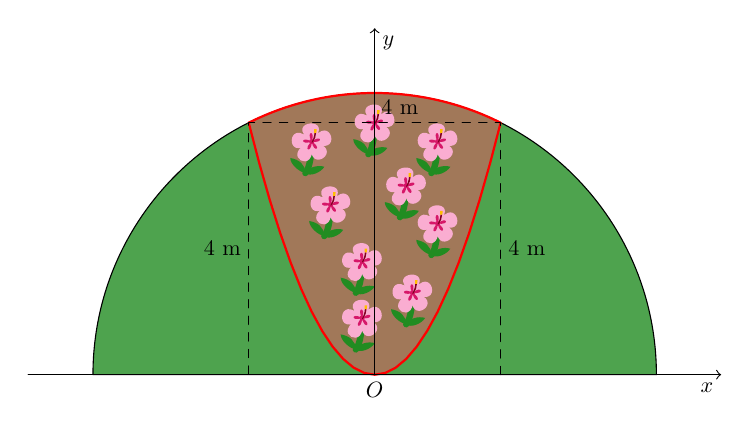
\begin{tikzpicture}[line join=round, line cap=round,scale=.8,transform shape]
				\definecolor{lavenderpink}{rgb}{0.98, 0.68, 0.82}
				\definecolor{dogwoodrose}{rgb}{0.84, 0.09, 0.41}
				\definecolor{burgundy}{rgb}{0.5, 0.0, 0.13}
				\definecolor{citrine}{rgb}{0.89, 0.82, 0.04}
				\definecolor{amber}{rgb}{1.0, 0.75, 0.0}
				\definecolor{forestgreen(web)}{rgb}{0.13, 0.55, 0.13}%màu lá
				\definecolor{chamoisee}{rgb}{0.63, 0.47, 0.35}
				%\clip (-4,-1) rectangle (4,4);
				
				%\def\r{3}
				\def\R{4}
				\pgfmathsetmacro{\r}{sqrt{20}}
				\path
				(0,0) coordinate (O);
				\def\xa{2}
				\def\ya{4}
				\def\xb{-2}
				\def\yb{4}
				\pgfmathsetmacro{\thetaA}{atan2(\ya,\xa)}
				\pgfmathsetmacro{\thetaB}{atan2(\yb,\xb)}
				
				\draw[fill=forestgreen(web)!80](\r,0) arc (0:180:\r)--cycle;
				\draw[red,line width=1mm, thick, fill=chamoisee] (\thetaA:\r) arc (\thetaA:\thetaB:\r)--plot[domain=-2:2] ({\x}, {(\x)^2});
				
				\tikzset{hoa/.pic={
						\def\L{
							(-.5,-2.5)
							..controls +(70:.5) and +(160:.5) .. (1,-2)
							..controls +(-120:.5) and +(-40:.5) .. cycle
							
							(-.5,-2.5)
							..controls +(90:.7) and +(-10:.7) .. (-1.7,-1.3)
							..controls +(-90:.5) and +(170:.5) .. cycle
							;}
						%\draw \L;
						\fill[forestgreen(web)] \L;
						
						\draw[forestgreen(web),line width=.8mm] (0,0)
						..controls +(-90:.8) and +(50:.6) .. (-.5,-2.5)
						%..controls +(-130:.6) and +(50:.2) .. (-1.5,-3.5)
						;
						\def\M{
							(0,0)..controls +(145:3) and +(45:3) ..(0,0)
							(0,0)..controls +(60:3) and +(-30:3) ..(0,0)
							(0,0)..controls +(-10:3) and +(-100:3) ..(0,0)
							(0,0)..controls +(-80:3) and +(-160:3) ..(0,0)
							(0,0)..controls +(-140:3) and +(-230:3) ..(0,0)
							;
						}
						\fill[lavenderpink] \M;
						%\draw[black]\M;
						\def\N{
							(0,0)..controls +(120:1) and +(70:1) ..(0,0)
							(0,0)..controls +(-10:1) and +(40:1) ..(0,0)
							(0,0)..controls +(-30:1) and +(-80:1) ..(0,0)
							(0,0)..controls +(-90:1) and +(-140:1) ..(0,0)
							(0,0)..controls +(150:1) and +(200:1) ..(0,0)
							;
						}
						%\draw[black]\N;
						\fill[dogwoodrose] \N;
						\fill[dogwoodrose](0,0) circle (6pt);
						
						\def\A{
							(0,-.03)..controls +(-120:.1) and +(-120:.1) ..(.1,-.03)
							..controls +(60:.3) and +(-90:.3) ..(.35,.7)--(.22,.7)
							..controls +(-90:.3) and +(60:.1) ..cycle;
						}
						\fill[burgundy] \A;
						%\draw[black]\A;
						
						\def\V{
							(.2,.7)
							..controls +(-10:.1) and +(-170:.1) ..(.37,.7)
							..controls +(80:.1) and +(-80:.1) ..(.4,1)
							..controls +(150:.1) and +(30:.1) ..(.2,1)
							..controls +(-110:.1) and +(90:.1) ..cycle;
						}
						\fill[amber] \V;
						%\draw[black]\V;
						
				}}
				
				\foreach \i/\j in{-.2/.9,-.2/1.8,.6/1.3,-.7/2.7,1/2.4,.5/3,-1/3.7,1/3.7,0/4}{
					\path
					(\i,\j)pic[scale=.2]{hoa};
				}
				
				\draw[dashed] (2,0)--(2,4)--(-2,4)--(-2,0);
				\draw[->] (-5.5,0)--(5.5,0)node[below left]{$x$};
				\draw[->] (0,0)node[below]{$O$}--(0,5.5)node[below right]{$y$};
				\draw[fill=black] (0,0) circle;
				%\node[below] at ($(S')!.5!(O')$) {$12$ m};
				\node[above] at (.4,4) {$4$ m};
				\node[left] at (-2,2) {$4$ m};
				\node[right] at (2,2) {$4$ m};
			\end{tikzpicture}
		\end{center}
		Chọn hệ trục tọa độ như hình vẽ. \\
		Phương trình đường tròn $(C)\colon x^2+y^2=20$ suy ra phương trình nửa trên đường tròn là $y=\sqrt{20-x^2}$.\\
		Parabol có đỉnh gốc $O$ và đi qua điểm $(2;4)$ nên phương trình $(P)\colon y=x^2$.\\
		Khi đó diện tích phần trồng hoa \[S=\displaystyle\int\limits_{-2}^{2} {\left(\sqrt{20-x^2}-x^2\right)}\mathrm{\,d}x\approx 11{,}94\mathrm{m}^2.\]
		Diện tích phần trồng cỏ là \[S'=\dfrac{\pi \cdot 20}{2}-S=10\pi-S.\]
		Số tiền để trồng hoa và trồng cỏ là
		\[S\cdot 150+S'\cdot 100\approx 3{,}74\text{ (triệu đồng)}.\]
	}
\end{ex}
\begin{ex} %Câu 6
	Năm $2016$, trong chiến dịch mang tên \lq\lq Niềm tự hào cuối cùng của loài người\rq\rq, kỳ thủ cờ vây số một thế giới Lee Sedol đã có trận đấu lịch sử với trí tuệ nhân tạo AlphaGo. Một trò chơi mô phỏng trận đấu này có luật như sau: Điểm khởi đầu của kỳ thủ là $2$. Trong mỗi ván đấu, nếu thắng kỳ thủ được cộng $1$ điểm, nếu hòa điểm số không thay đổi, nếu thua bị trừ $1$ điểm. Trận đấu kết thúc ngay khi kỳ thủ đạt $3$ điểm (giành chiến thắng) hoặc $0$ điểm (thất bại). Giả sử xác suất mỗi ván thắng, hòa, thua của kỳ thủ lần lượt là $\dfrac{1}{4}$, $\dfrac{1}{4}$, $\dfrac{1}{2}$ và kết quả các ván đấu là độc lập với nhau. Xác suất để trận đấu kết thúc sau đúng $6$ ván và kỳ thủ là người giành chiến thắng là $p$. Tính $4096p$.
	\par
	\shortans{41}
	\loigiai{
	}
\end{ex}